\section{Methodology}

The methodology of this lab exercise follows the usual process for machine learning problems/researches
\[
  \text{data} \to \text{preprocessing} \to \text{modeling} \to \text{evaluation}
\]

The preprocessing section mainly consists of splitting the dataset into training and testing data, checking the validity of data, as well as many others. The Convolutional Neural Network, like other neural networks, can be customized especially in the number of convolutional layers, different pooling methods, different kernels, etc. Unlike previous models, there really isn't much customization that could be done to them other than the hyperparameters to alter slightly how it works. But when it comes to CNNs, there's a lot more room for varying techniques. 

Later in experimentation, we will see how customizing the CNN can affect performance for detecting these hair types. For evaluation, the accuracy metric is used to measure the model's performance. 

\subsection{Data Acquisition and Preparation}

\subsubsection{Loading of Images}

A folder named 'hair_types' was manually imported in the repository containing 1000 images. Inside that folder has subdirectories for each hair type. Python Imaging Library (PIL) library was used to create a custom function of validating the images that was imported. It ensures that none of these images are corrupted and adhere to specific formats, such as PNG, JPG, and BMP. We exclude files that are not accepted by Tensorflow and does not match the specific formats, such as .WebP. After loading these images, 14 images were deleted and one image with a file type of .gif was also detected, but we didn't remove it because it is still valid for this experiment. This step is important to minimize potential issues during model training.

\subsubsection{Image Categorization}

This step involves segrating the images into three groups based on hair type labels found in their file paths. This will help in the structured training of the model by defining the classes of each images.

\subsubsection{Manual Inspection}

To ensure that no invalid images were overlooked, we manually inspected the images through file explorer. Through this inspection, it was detected that there is one image in 'Straight_Hair' subdirectory that is just a microphone logo. Thus, excluding this is beneficial to prevent the model learning unnecessary and wrong information.

\subsubsection{Image Display}

Using matplotlib, we displayed a sample from each category. This step is important to ensure the integrity and appropriateness of the labels and the image themselves.

\subsection{Preprocessing}

\subsubsection{Data Augmentation}

Initaially, we tried applying several data augmentation technicques, such as random horizontal and vertical flips, random rotations, and random zooms. However, we didn't apply data augmentation in the final model, which will be discussed on the Experiments section.

\subsubsection{Splitting Dataset}

To ensure generalizability of this model, we utilized Tensorflow's `image_dataset_from_directory` method to split the image data into training and validation datasets. 20 percent of the data was allocated for validation. Additionally, we resize all images to a uniform `(256,256)' for consistency and batch them in sizes of 64. Splitting the data this way helps prevent overfitting by ensuring that the model does not memoreize the training data and allows us to fine-tune the model parameters based on the performance metrics gathered from validation set.

\subsubsection{Sobel Edge Detection}

A custom preprocessing function was created to detect Sobel edges in the images. This technique highlights the edges within each image. This technique will be applied for both training sets and validation sets to ensure consistency in how images are presented to the model.

We generated 9 samples from the dataset to display sobel edges applied images.

\begin{figure}[H]
  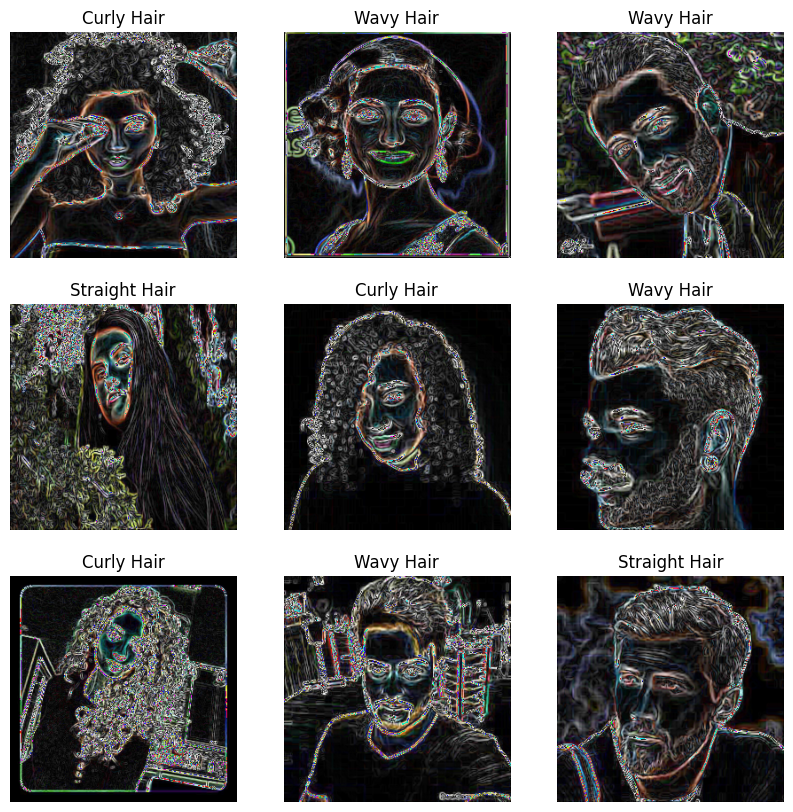
\includegraphics[width=\linewidth]{figures/sobel_edge_images.png}
  \caption{Hair Types Example with Sobel Edge}
  \label{fig:hairtypes}
\end{figure}

\subsection{Modeling}

\subsubsection{Convolutional Neural Network Architecture}

In this step, we constructed a convolutional neural network (CNN) model using the Keras library's `Sequential` API. We also normalized the input images by the `Rescaling` layer to scale pixel values to a range of 0 to 1, since the pixel values of the images range from 0 to 255 because of the colors. This normalization will help the model learn more efficiently, since neural networks perform better with small input values.

% discuss convolution layers here and what hyperparameters were used
% discuss activation functions
% discuss batch normalization
%  discuss pooling and dropout
%  discuss flattening and dense layers

\subsubsection{Training the Model}

% discuss the compilation of the model with Adam optimizer and categorical cross entropy loss

% discuss the training both training and validation datasets and what is the final results

\begin{figure}[H]
  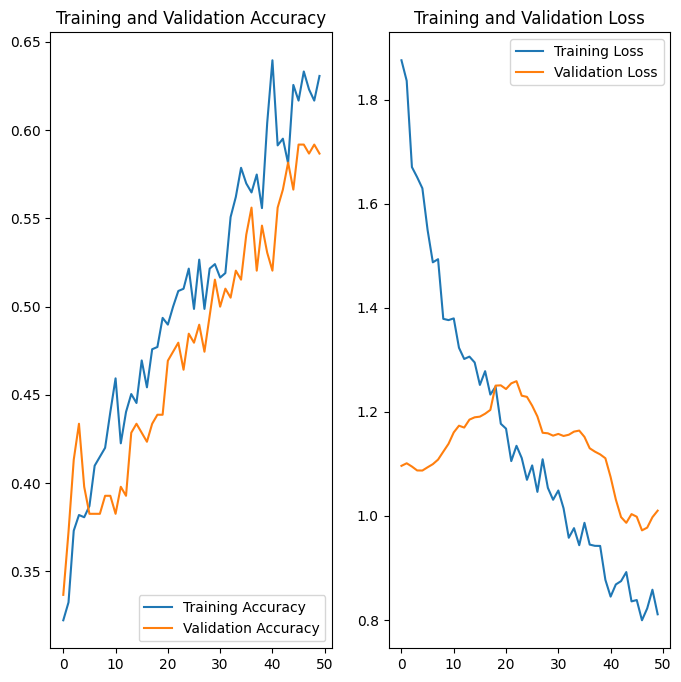
\includegraphics[width=\linewidth]{figures/training_validation_results.png}
  \caption{Training and Validation Results}
  \label{fig:results}
\end{figure}

\subsection{Evaluation}

% discuss the use of line graph to analyze training and validation
% discuss the use of confusion matrix
% discuss the use of classification report
%  discuss the use of model prediction in one sample
